\subsection{The Life Cycle of an SGX Thread}
\label{sec:sgx_threads}

Between the time when an enclave is
initialized~(\S~\ref{sec:sgx_einit_overview}) and the time when it is torn
down~(\S~\ref{sec:sgx_eremove}), the enclave's code can be executed by any
application process that has the enclave's EPC pages mapped into its virtual
address space.

% Internal CREGs: SDM S 41.1.4
% Access Control Requirements: SDM S 38.3

When executing the code inside an enclave, a logical processor is said to be
\textit{in enclave mode}, and the code that it executes can access the
regular~(PT\_REG,~\S~\ref{sec:sgx_epcm}) EPC pages that belong to the currently
executing enclave. When a logical process is outside enclave mode, it bounces
any memory accesses inside the Processor Reserved Memory
range~(PRM,~\S~\ref{sec:sgx_prm}), which includes the EPC.

Each logical processor that executes enclave code uses a Thread Control
Structure~(TCS,~\S~\ref{sec:sgx_tcs}). When a TCS is used by a logical
processor, it is said to be \textit{busy}, and it cannot be used by any other
logical processor.  Figure~\ref{fig:sgx_tcs_lifecycle} illustrates the
instructions used by a host process to execute enclave code and their
interactions with the TCS that they target.

\begin{figure}[hbt]
  \centering
  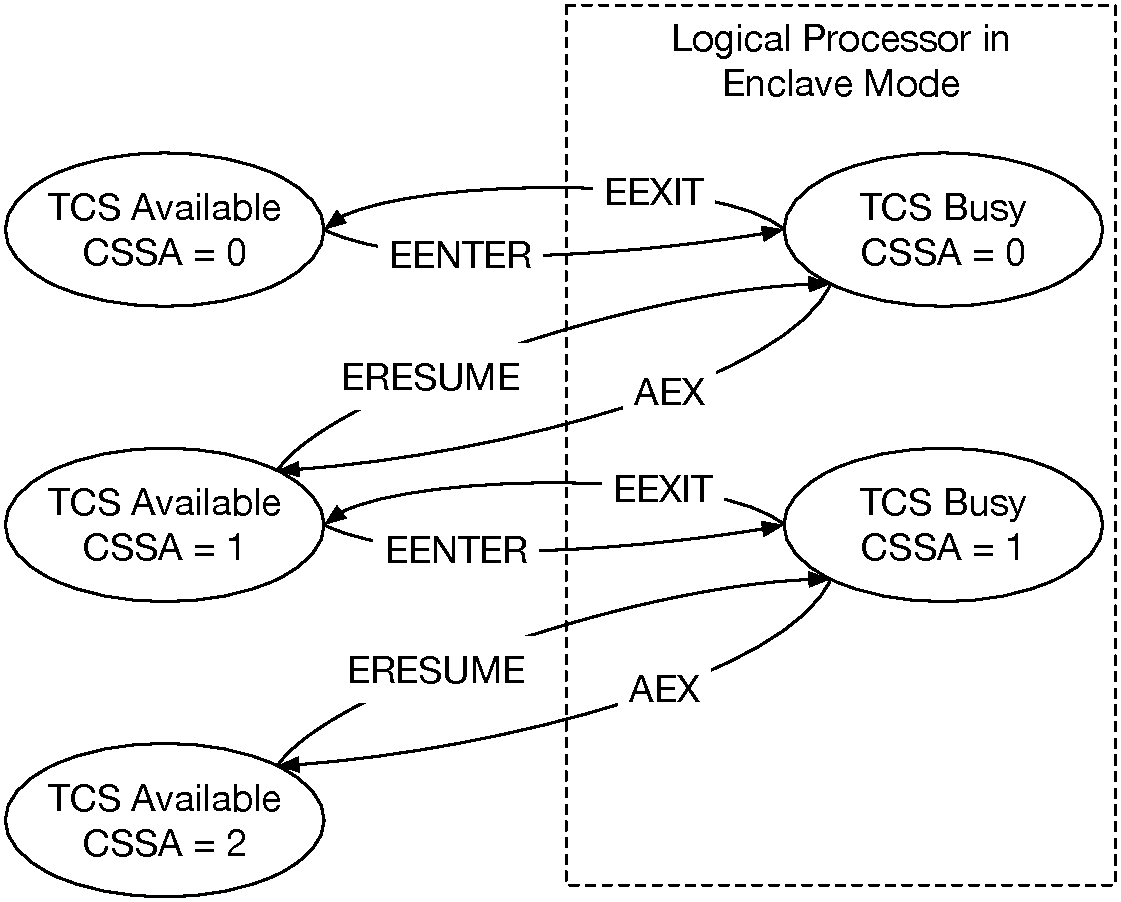
\includegraphics[width=75mm]{figures/sgx_tcs_lifecycle.pdf}
  \caption{
    The stages of the life cycle of an SGX Thread Control Structure (TCS) that
    has two State Save Areas (SSAs).
  }
  \label{fig:sgx_tcs_lifecycle}
\end{figure}

Assuming that no hardware exception occurs, an enclave's host process uses the
\texttt{EENTER} instruction, described in \S~\ref{sec:sgx_eenter}, to execute
enclave code. When the enclave code finishes performing its task, it uses the
\texttt{EEXIT} instruction, covered in \S~\ref{sec:sgx_eexit}, to return the
execution control to the host process that invoked the enclave.

If a hardware exception occurs while a logical processor is in enclave mode,
the processor is taken out of enclave mode using an
\textit{Asynchronous Enclave Exit}~(AEX), summarized in \S~\ref{sec:sgx_aex},
before the system software's exception handler is invoked. After the system
software's handler is invoked, the enclave's host process can use the
\texttt{ERESUME} instruction, described in \S~\ref{sec:sgx_eresume}, to
re-enter the enclave and resume the computation that it was performing.


\subsubsection{Synchronous Enclave Entry}
\label{sec:sgx_enclave_mode}
\label{sec:sgx_eenter}

At a high level, \texttt{EENTER} performs a controlled jump into enclave code,
while performing the processor configuration that is needed by SGX's security
guarantees. Going through all the configuration steps is a tedious exercise,
but it a necessary prerequisite to understanding how all data structures used
by SGX work together. For this reason, \texttt{EENTER} and its siblings are
described in much more detail than the other SGX instructions.

% ENCLU - Execute an Enclave User Function of Specified Leaf Number: SDM S 41.2

\texttt{EENTER}, illustrated in Figure~\ref{fig:sgx_eenter} can only be
executed by unprivileged application software running at ring
3~(\S~\ref{sec:rings}), and results in an undefined instruction (\#UD) fault if
is executed by system software.

\begin{figure}[hbt]
  \centering
  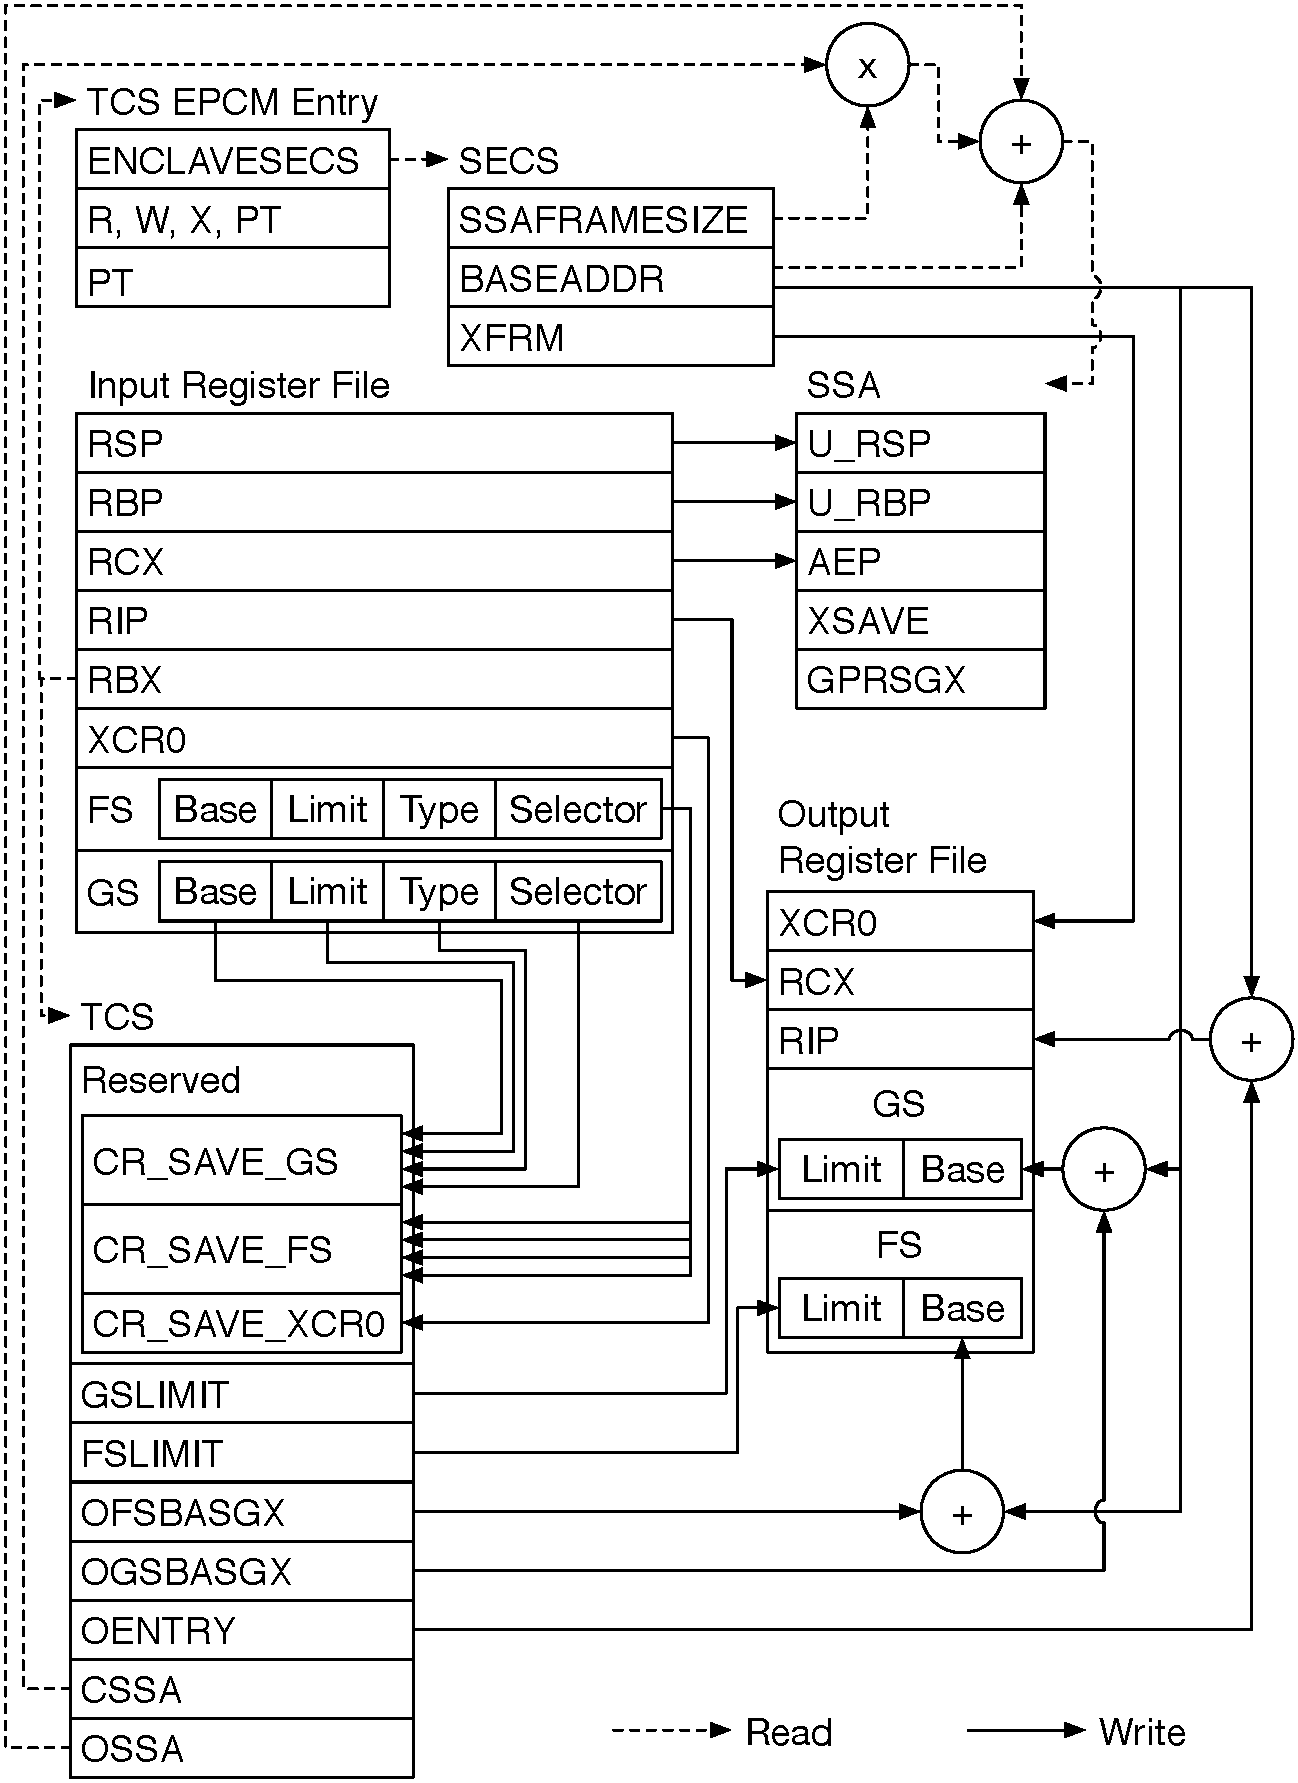
\includegraphics[width=87mm]{figures/sgx_eenter.pdf}
  \caption{
    Data flow diagram for a subset of the logic in \texttt{EENTER}. The figure
    omits the logic for disabling debugging features, such as hardware
    breakpoints and performance monitoring events.
  }
  \label{fig:sgx_eenter}
\end{figure}

\texttt{EENTER} switches the logical processor to enclave mode, but does not
perform a privilege level switch~(\S~\ref{sec:faults}). Therefore, enclave code
always executes at ring 3, with the same privileges as the application code
that calls it. This makes it possible for an infrastructure owner to allow
user-supplied software to create and use enclaves, while having the assurance
that the OS kernel and hypervisor can still protect the infrastructure from
buggy or malicious software.

% EENTER - Enters an Enclave: SDM S 41.4.1
% Current State Save Area Frame (CSSA): SDM S 38.8.3
% Number of State Save Area Frames (NSSA): SDM S 38.8.4

\texttt{EENTER} takes the virtual address of a TCS as its input, and requires
that the TCS is \textit{available} (not busy), and that at least one State Save
Area~(SSA,~\S~\ref{sec:sgx_ssa}) is available in the TCS. The latter check is
implemented by making sure that the \textit{current SSA index}~(CSSA) field in
the TCS is less than the number of SSAs (NSSA) field. The SSA indicated by the
CSSA, which shall be called the \textit{current SSA}, is used in the event that
a hardware exception occurs while enclave code is executed.

\texttt{EENTER} transitions the logical processor into enclave mode, and sets
the instruction pointer (RIP) to the value indicated by the \textit{entry point
offset}~(OENTRY) field in the TCS that it receives. \textit{EENTER} is used by
an untrusted caller to execute code in a protected environment, and therefore
has the same security considerations as
\texttt{SYSCALL}~(\S~\ref{sec:privilege_switches}), which is used to call into
system software. Setting RIP to the value indicated by OENTRY guarantees to the
enclave author that the enclave code will only be invoked at well defined
points, and prevents a malicious host application from bypassing any security
checks that the enclave author may perform.

% Interactions with the Processor Extended State and Misc State: SDM S 42.7
% SECS.ATTRIBUTES.XFRM: SDM S 42.7.2.1

\texttt{EENTER} also sets XCR0~(\S~\ref{sec:registers}), the register that
controls which extended architectural features are in use, to the value of the
XFRM enclave attribute~(\S~\ref{sec:sgx_secs_attributes}). Ensuring that XCR0 is
set according to the enclave author's intentions prevents a malicious operating
system from bypassing an enclave's security by enabling architectural features
that the enclave is not prepared to handle.

Furthermore, \texttt{EENTER} loads the bases of the segment
registers~(\S~\ref{sec:segments}) FS and GS using values specified in the TCS.
The segments' selectors and types are hard-coded to safe values for ring 3 data
segments. This aspect of the SGX design makes it easy to implement per-thread
Thread Local Storage (TLS). For 64-bit enclaves, this is a convenience feature
rather than a security measure, as enclave code can securely load new bases
into FS and GS using the \texttt{WRFSBASE} and \texttt{WRGSBASE} instructions.

The \texttt{EENTER} implementation backs up the old values of the registers
that it modifies, so they can be restored when the enclave finishes its
computation. Just like \texttt{SYSCALL}, \texttt{EEENTER} saves the address of
the following instruction in the RCX register.

Interestingly, the SDM states that the old values of the XCR0, FS, and GS
registers are saved in new registers dedicated to the SGX implementation.
However, given that they will only be used on an enclave exit, we expect that
the registers are saved in DRAM, in the reserved area in the TCS.

Like \texttt{SYSCALL}, \texttt{EENTER} does not modify the stack pointer
register (RSP). To avoid any security exploits, enclave code should set RSP to
point to a stack area that is entirely contained in EPC pages. Multi-threaded
enclaves can easily implement per-thread stack areas by setting up each
thread's TLS area to include a pointer to the thread's stack, and by setting
RSP to the value obtained by reading the TLS area at which the FS or GS segment
points.

Last, when \texttt{EENTER} enters enclave mode, it suspends some of the
processor's debugging features, such as hardware breakpoints and Precise Event
Based Sampling~(PEBS). Conceptually, a debugger attached to the host process
sees the enclave's execution as one single processor instruction.


\subsubsection{Synchronous Enclave Exit}
\label{sec:sgx_eexit}

% EEXIT - Exits an Enclave: SDM S 41.4.1

\texttt{EEXIT} can only be executed while the logical processor is in enclave
mode, and results in a (\#UD) if executed in any other circumstances. In a
nutshell, the instruction returns the processor to ring 3 outside enclave mode
and restores the registers saved by \texttt{EENTER}, which were described above.

Unlike \texttt{SYSRET}, \texttt{EEXIT} sets RIP to the value read from RBX,
after exiting enclave mode. This is inconsistent with \texttt{EENTER}, which
saves the RIP value to RCX. Unless this inconsistency stems from an error in
the SDM, enclave code must be sure to note the difference.

The SDM explicitly states that \texttt{EEXIT} does not modify most registers,
so enclave authors must make sure to clear any secrets stored in the
processor's registers before returning control to the host process.
Furthermore, enclave software will most likely cause a fault in its caller if
it doesn't restore the stack pointer RSP and the stack frame base pointer RBP
to the values that they had when \texttt{EENTER} was called.

It may seem unfortunate that enclave code can induce faults in its caller.
For better or for worse, this perfectly matches the case where an application
calls into a dynamically loaded module. More specifically, the module's code is
also responsible for preserving stack-related registers, and a buggy module
might jump anywhere in the application code of the host process.

At first glance, it may seem elegant to have \texttt{EENTER} store the contents
of the XCR0, FS, and GS registers in the current SSA, and have \texttt{EEXIT}
restore them from the current SSA. However, this approach would break the Intel
architecture's guarantees that only system software can modify XCR0, and
application software can only load segment registers using selectors that index
into the GDT or LDT set up by system software (\S~\ref{sec:segments}).
Specifically, a malicious application could modify these privileged registers
by creating an enclave that writes the desired values to the current SSA
locations backing up the registers, and then executes \texttt{EEXIT}.

This section describes the \texttt{EENTER} behavior for 64-bit enclaves. The
\texttt{EENTER} implementation for 32-bit enclaves is significantly more
complex, due to the extra special cases introduced by the full-fledged
segmentation model that is still present in the 32-bit Intel architecture. As
stated in the introduction, we are not interested in such legacy aspects.


\subsubsection{Asynchronous Enclave Exit (AEX)}
\label{sec:sgx_aex}

If a hardware exception, like a fault~(\S~\ref{sec:faults}) or an
interrupt~(\S~\ref{sec:interrupts}), occurs while a logical processor is
executing an enclave's code, the processor performs an
\textit{Asynchronous Enclave Exit}~(AEX) before invoking the system software's
exception handler, as shown in Figure~\ref{fig:sgx_aex_setup}.

\begin{figure}[hbt]
  \centering
  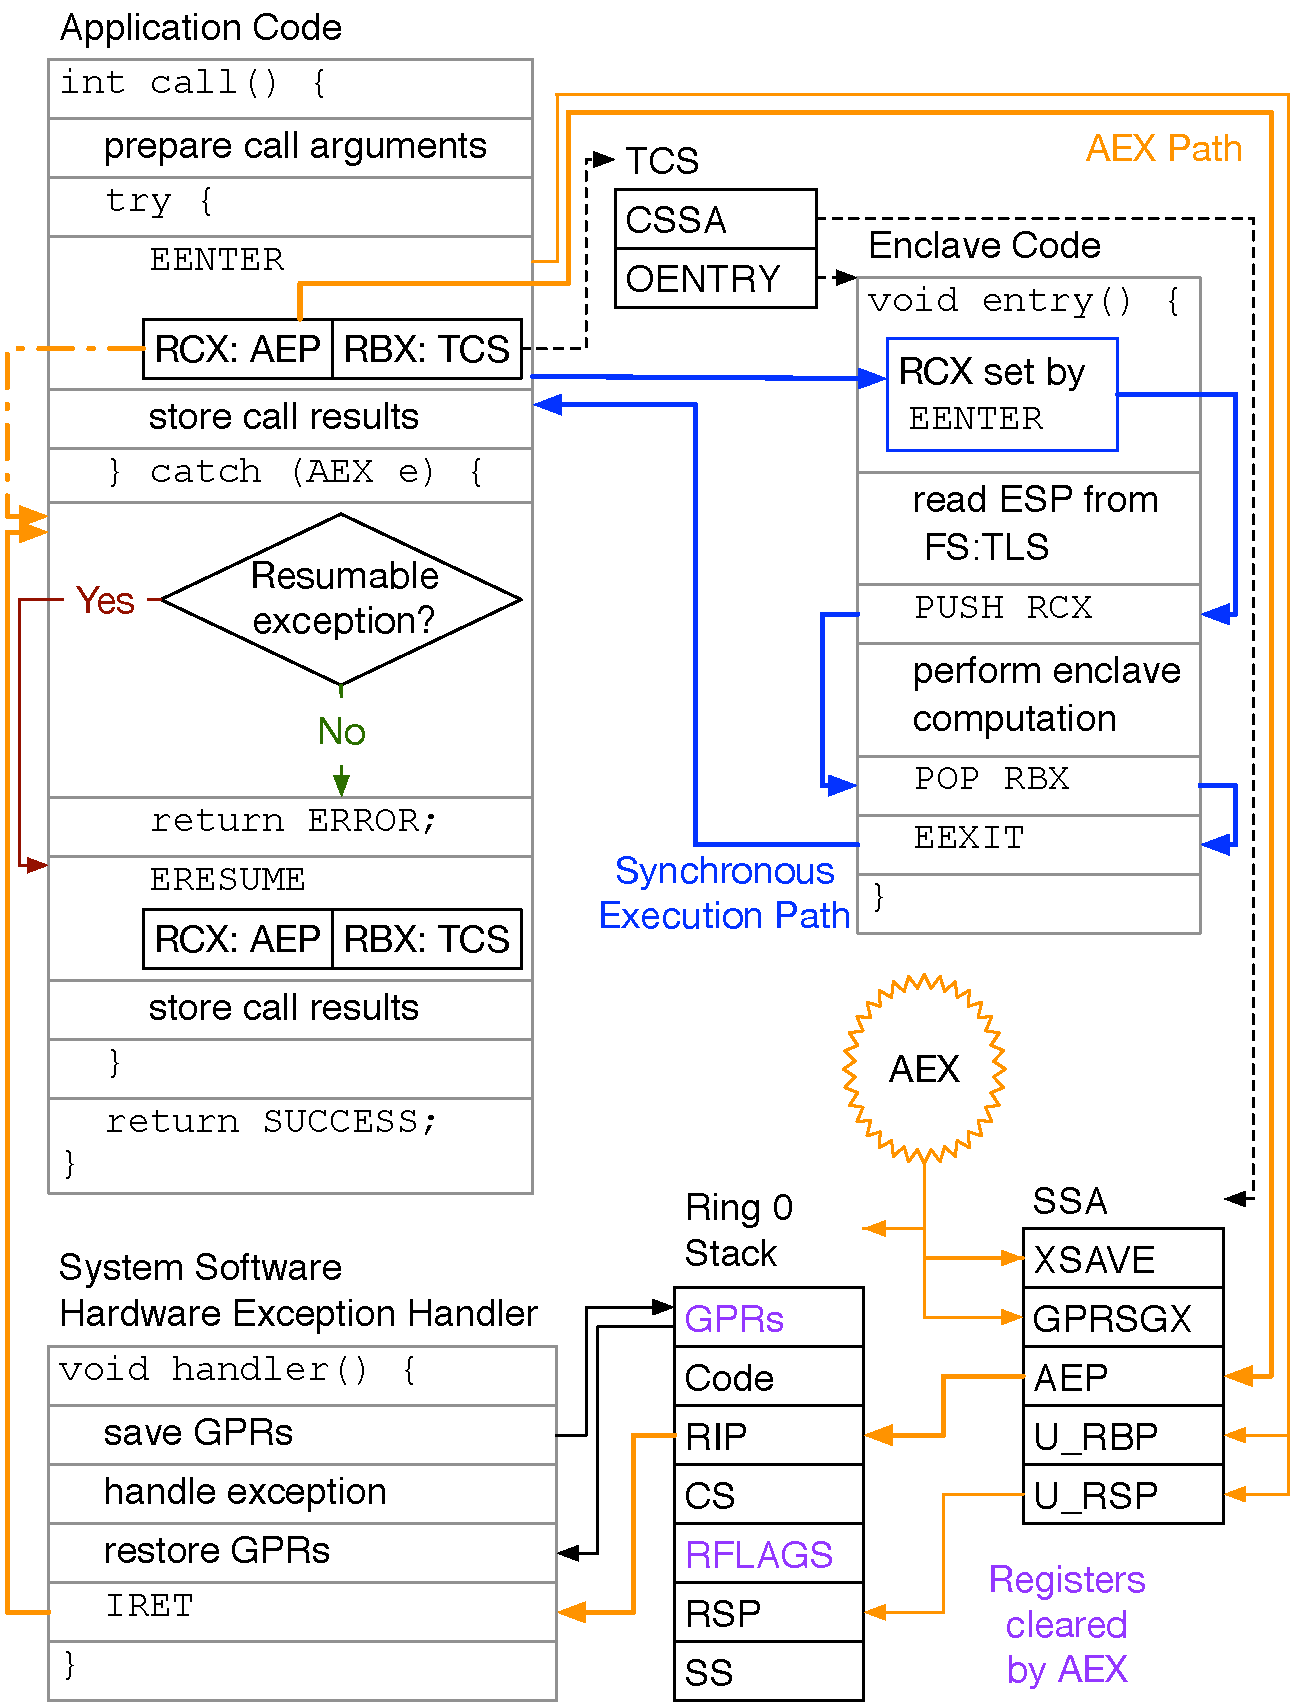
\includegraphics[width=87mm]{figures/sgx_aex_setup.pdf}
  \caption{
    If a hardware exception occurs during enclave execution, the synchronous
    execution path is aborted, and an Asynchronous Enclave Exit (AEX) occurs
    instead.
  }
  \label{fig:sgx_aex_setup}
\end{figure}

% AEX Flow: SDM S 40.4
% AEX Operational Detail: SDM S 40.4.1

The AEX saves the enclave code's execution context~(\S~\ref{sec:registers}),
restores the state saved by \texttt{EENTER}, and sets up the processor
registers so that the system software's hardware exception handler will return
to an \textit{asynchronous exit handler} in the enclave's host process. The
exit handler is expected to use the \texttt{ERESUME} instruction to resume the
enclave computation that was interrupted by the hardware exception.

Asides from the behavior described in \S~\ref{sec:sgx_eenter}, \texttt{EENTER}
also writes some information to the current SSA, which is only used if an AEX
occurs. As shown in Figure~\ref{fig:sgx_eenter}, \texttt{EENTER} stores the
stack pointer register RSP and the stack frame base pointer register RBP into
the U\_RSP and U\_RBP fields in the current SSA. Last, \texttt{EENTER} stores
the value in RCX in the \textit{Asynchronous Exit handler Pointer}~(AEP) field
in the current SSA.

When a hardware exception occurs in enclave mode, the SGX implementation
performs a sequence of steps that takes the logical processor out of enclave
mode and invokes the hardware exception handler in the system software.
Conceptually, the SGX implementation first performs an AEX to take the logical
processor out of enclave mode, and then the hardware exception is handled
using the standard Intel architecture's behavior described in
\S~\ref{sec:faults}. Actual Intel processors may interleave the AEX
implementation with the exception handling implementation. However, for
simplicity, this work describes AEX as a separate process that is performed
before any exception handling steps are taken.

In the Intel architecture, if a hardware exception occurs, the application
code's execution context can be read and modified by the system software's
exception handler (\S~\ref{sec:faults}). This is acceptable when the system
software is trusted by the application software. However, under SGX's threat
model, the system software is not trusted by enclaves. Therefore, the AEX step
erases any secrets that may exist in the execution state by resetting all its
registers to predefined values.

% State Saving by AEX: SDM S 40.2

Before the enclave's execution state is reset, it is backed up inside the
current SSA. Specifically, an AEX backs up the general purpose
registers~(GPRs,~\S~\ref{sec:registers}) in the GPRSGX area in the SSA, and
then performs an \texttt{XSAVE}~(\S~\ref{sec:registers}) using the
requested-feature bitmap (RFBM) specified in the XFRM field in the enclave's
SECS. As each SSA is entirely stored in EPC pages allocated to the enclave, the
system software cannot read or tamper with the backed up execution state. When
an SSA receives the enclave's execution state, it is marked as used by
incrementing the CSSA field in the current TCS.

% Compatible Switch to the Exiting Stack of AEX: SDM S 40.1

After clearing the execution context, the AEX process sets RSP and RBP to the
values saved by \texttt{EENTER} in the current SSA, and sets RIP to the value
in the current SSA's AEP field. This way, when the system software's hardware
exception handler completes, the processor will execute the asynchronous exit
handler code in the enclave's host process. The SGX design makes it easy to
set up the asynchronous handler code as an exception handler in the routine
that contains the \texttt{EENTER} instruction, because the RSP and RBP
registers will have the same values as they had when \texttt{EENTER} was
executed.

Many of the actions taken by AEX to get the logical processor outside of
enclave mode match \texttt{EEXIT}. The segment registers FS and GS are restored
to the values saved by \texttt{EENTER}, and all the debugging facilities that
were suppressed by \texttt{EENTER} are restored to their previous states.


\subsubsection{Recovering from an Asynchronous Exit}
\label{sec:sgx_eresume}

When a hardware exception occurs inside enclave mode, the processor performs
an AEX before invoking the exception's handler set up by the system software.
The AEX sets up the execution context in such a way that when the system
software finishes processing the exception, it returns into an asynchronous
exit handler in the enclave's host process. The asynchronous exception handler
usually executes the \texttt{ERESUME} instruction, which causes the logical
processor to go back into enclave mode and continue the computation that was
interrupted by the hardware exception.

\texttt{ERESUME} shares much of its functionality with \texttt{EENTER}. This is
best illustrated by the similarity between Figures
\ref{fig:sgx_aex_eresume} and \ref{fig:sgx_aex_setup}.

\begin{figure}[hbt]
  \centering
  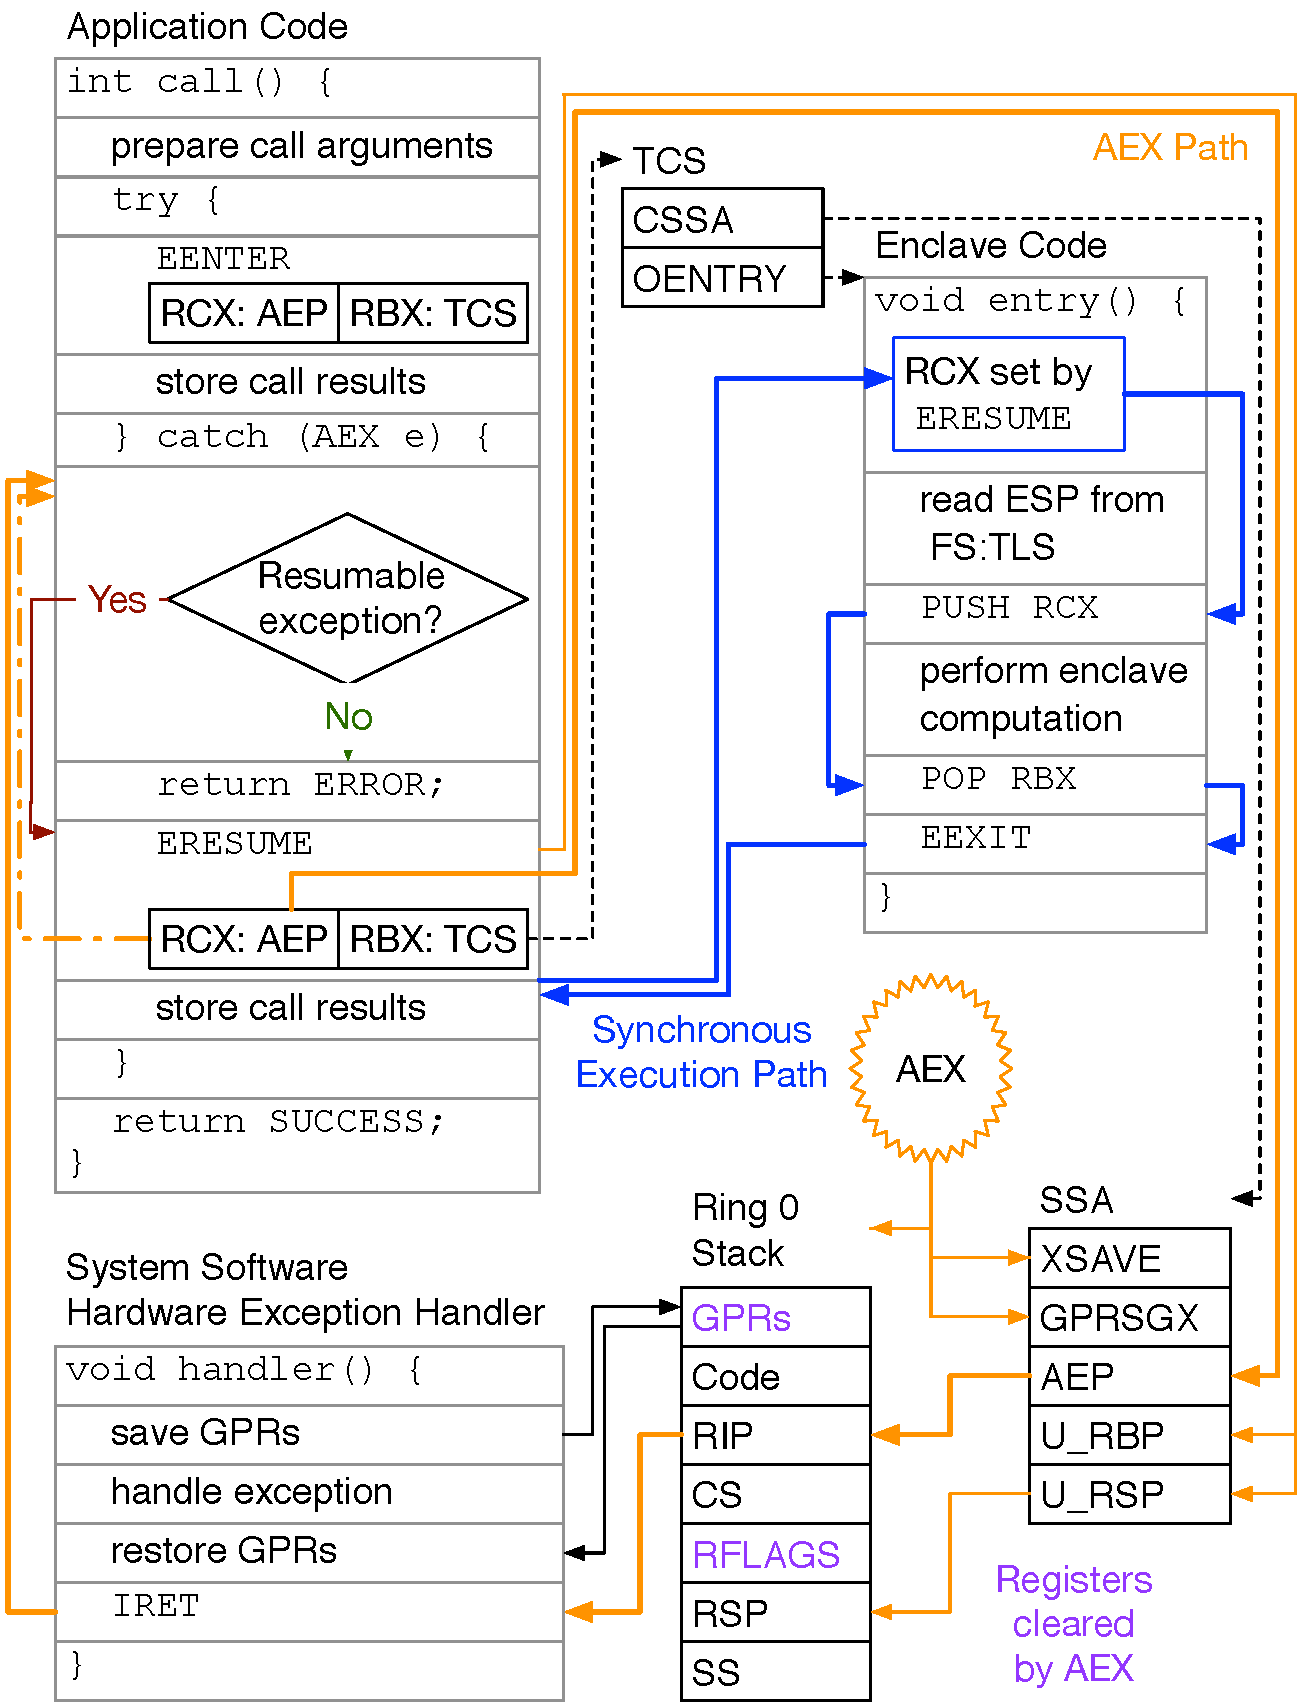
\includegraphics[width=87mm]{figures/sgx_aex_eresume.pdf}
  \caption{
    If a hardware exception occurs during enclave execution, the synchronous
    execution path is aborted, and an Asynchronous Enclave Exit (AEX) occurs
    instead.
  }
  \label{fig:sgx_aex_eresume}
\end{figure}

\texttt{EENTER} and \texttt{ERESUME} receive the same inputs, namely a pointer
to a TCS, described in \S~\ref{sec:sgx_eenter}, and an AEP, described in
\S~\ref{sec:sgx_aex}. The most common application design will pair each
\texttt{EENTER} instance with an asynchronous exit handler that invokes
\texttt{ERESUME} with exactly the same arguments.

The main difference between \texttt{ERESUME} and \texttt{EENTER} is that the
former uses an SSA that was ``filled out'' by an AEX~(\S~\ref{sec:sgx_aex}),
whereas the latter uses an empty SSA. Therefore, \texttt{ERESUME} results in a
\#GP fault if the CSSA field in the provided TCS is 0 (zero), whereas
\texttt{EENTER} fails if CSSA is greater than or equal to NSSA.

When successful, \texttt{ERESUME} decrements the CSSA field of the TCS, and
restores the execution context backed up in the SSA pointed to by the CSSA field
in the TCS. Specifically, the \texttt{ERESUME} implementation restores the
GPRs~(\S~\ref{sec:registers}) from the GPRSGX field in the SSA, and performs an
\texttt{XRSTOR}~(\S~\ref{sec:registers}) to load the execution state
associated with the extended architectural features used by the enclave.

\texttt{ERESUME} shares the following behavior with
\texttt{EENTER}~(\S~\ref{sec:sgx_eenter}). Both instructions write the U\_RSP,
U\_RBP, and AEP fields in the current SSA. Both instructions follow the same
process for backing up XCR0 and the FS and GS segment registers, and set them
to the same values, based on the current TCS and its enclave's SECS. Last, both
instructions disable the same subset of the logical processor's debugging
features.

An interesting edge case that \texttt{ERESUME} handles correctly is that it
sets XCR0 to the XFRM enclave attribute \textbf{before} performing an
\texttt{XRSTOR}. It follows that \texttt{ERESUME} fails if the requested
feature bitmap (RFBM) in the SSA is not a subset of XFRM. This matters because,
while an AEX will always use the XFRM value as the RFBM, enclave code executing
on another thread is free to modify the SSA contents before \texttt{ERESUME} is
called.

The correct sequencing of actions in the \texttt{ERESUME} implementation
prevents a malicious application from using an enclave to modify registers
associated with extended architectural features that are not declared in XFRM.
This would break the system software's ability to provide thread-level
execution context isolation.
